%
%
\documentclass{article}
\usepackage{amsmath}
\usepackage{graphicx}
\usepackage{color}
\usepackage{caption}
\usepackage{amsfonts}
%\usepackage[margin=3cm]{geometry}
\usepackage{tikz}
\newcommand{\bs}{\boldsymbol}                               %

\begin{document}

\title{Numerical methods}
\author{Dominic Skinner}
\maketitle

Consider the govering equations
\begin{equation}\label{eq1}
\left( \begin{array}{c} p(z) \\ 0 \end{array} \right) =
 \left( \begin{array}{c} \sigma_y \\ \tau_{xy} \end{array} \right) =
\int_0^{\infty} \left(
\begin{array}{cc} K_{11}(x-z) & K_{12}(x-z) \\ K_{21}(x-z) & K_{22}(x-z) \end{array}
\right)
 \left( \begin{array}{c} g'(x) \\ h'(x) \end{array} \right) dx
\end{equation}
%
\begin{equation}\label{eq2}
h^2p'=\lambda
\end{equation}
Have the ``input'' parameters as 
\begin{itemize}
\item BC's $P$, $M$ (or equivalently $g'$, $h''$ at $x\to\infty$)
\item $\lambda$ , the speed
\end{itemize}
Want to solve for the toughness $K_I$ and $K_{II}$. In this project,
we have so far focused on $K_I$.
\begin{figure}[!ht]\centering
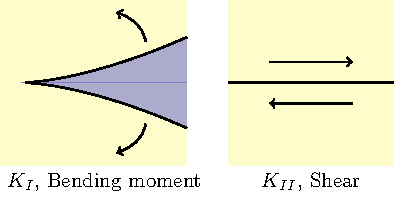
\includegraphics{NumFig3.pdf}
\end{figure}

\underline{Goal:} 
Find $\lambda$ such that $K_I(\lambda)=0$, ``Zero toughness solution''.
Given this we then want to investigate the behaviour for small $K_I\approx 0$.
To do this, take some given value of $\lambda$ and then solve equations
\ref{eq1}, \ref{eq2}.
\subsection*{Discretization of problem}
The method chosen to discretize the problem is to take a vector 
$(x_1, \dots , x_n)$ of $n$ points at which we measure $g', h'$ and have a 
vector $(z_1, \dots ,z_{n-1})$ of $n-1$ intermediate 
points at which $p$ is measured. (The spacing chosen is a $\tan^2$ spacing)
\begin{figure}[!ht]\centering
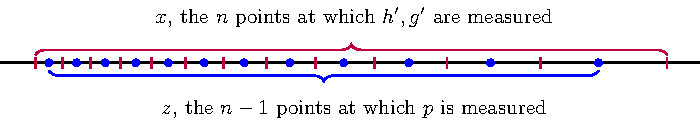
\includegraphics{NumFig2.pdf}
\end{figure}

The ``obvious'' way to interpolate $h'$ in between the $x_i$'s is 
simple linear interpolation. But both $h',g'$ become singular near 0.
However, we expect a $x^{-1/2}$ singularity, which allows us to ``remove''
said singularity. 
The interpolation used is
\[ g'(x) = \left\{ \begin{array}{cc} \frac{1}{\sqrt{x}}(a_ix+b_i) &
i <t \\ a_ix+b_i & i \geq t \end{array} \right. \]
for $x$ in the spline $x \in [x_i,x_{i+1}]$. Choose $1 < t < n$, typically
$t=n/2$. Similarly
\[ h'(x) = \left\{ \begin{array}{cc} \frac{1}{\sqrt{x}}(c_ix+d_i) &
i <t \\ c_ix+d_i & i \geq t \end{array} \right. \]
With the same $t$ used. We also define $a_n, b_n, c_n, d_n$ for interpolation
beyond $x_n$.

The values of $g',h'$ are stored via 
\[ \bs{\theta} = \left( \begin{array}{c} a_1x_1+b_1 \\ \vdots 
\\ a_n x_n+b_n \\[4pt] c_1x_1+d_1 \\ \vdots \\ c_n x_n + d_n \end{array} 
\right) \]
Once one has $\bs{\theta}$, it is trivial to recover, say $g'(x_i)$, since
either $g'(x_i) = \bs{\theta}_i$ or $g'(x_i) = \bs{\theta}_i/\sqrt{x_i}$.
Similarly, given $g'(x_i)$; $\bs{\theta}_i$ can be calculated.

\subsection*{Recovering the a$_{i}$'s}
Suppose we know $\bs{\theta}$, (and always assume we know the $x_i$).
Can we recover $a_i, b_i, c_i, d_i$? 
The answer is yes, once we add in the boundary conditions at $\infty$.
Further we have that 
\[ \bs{\gamma} = \left( \begin{array}{c} a_1 \\ \vdots 
\\ a_n \\[3pt] b_1 \\ \vdots \\ b_n \\[3pt] c_1 \\ \vdots \\ c_n 
\\[3pt] d_1 \\ \vdots \\ d_n  \end{array} \right)
= T \bs{\theta} \]
Where T is a $4n \times n$ interpolation matrix. A quick check reveals
we have $4n$ unknowns, in $\bs{\gamma}$. Knowing $\theta$ provides $2n$
equations. Demanding continuity of the interpolated $g',h'$ provides
another $2(n-1)$ equations, (match at $x_2, \dots, x_n$). Finally boundary
conditions on the spline at $\infty$ provide another 2 equations.

The continuity conditions are 
\begin{align*}
a_1 x_2 + b_1 &= a_2 x_2 + b_2 \\
& \;\; \vdots \\
a_{t-2} x_{t-1} + b_{t-2} &= a_{t-1} x_{t-1} + b_{t-1} \\
(a_{t-1} x_{t} + b_{t-1})/\sqrt{x_t} &= a_{t} x_{t} + b_{t} \\
a_{t} x_{t+1} + b_{t} &= a_{t+1} x_{t+1} + b_{t+1} \\
& \;\; \vdots \\
a_{n-1} x_{n} + b_{n-1} &= a_{n} x_{n} + b_{n} \\
\end{align*}
and similar for $c,d$. This means that with the exceptions of
$i=t-1,n$, have that 
\[ \frac{\theta_{i+1}-\theta_i}{x_{i+1}-x_i} = a_i \]
\[ \frac{\theta_{i}\,x_{i+1}-\theta_{i+1}x_i}{x_{i+1}-x_i} = b_i \]
Same idea with $x_{t-1}$, just have to be a little careful about
the switch in the continuity condition,
\[ \frac{\sqrt{x_t}\theta_{t}-\theta_{t-1}}{x_t-x_{t-1}} = a_{t-1} \]
\[ \frac{\theta_{t-1}\,x_t-\theta_t x_{t-1}\sqrt{x_t}}
{x_t-x_{t-1}} = b_{t-1} \]

So we are almost done, just missing 4 rows in our matrix. Have the
$n^{th}$ row as all zeros, i.e. $a_n=0$ due to boundary conditions,
and so trivially the $2n^{th}$ row is 0 except $T_{2n,n} = 1 $
Now, B.C. for $h'$ implies $h''(x_n) \approx h''(x_{n-1})$ i.e.
$c_n=c_{n-1}$ and thus from continuity $d_n=d_{n-1}$. This completes
our interpolation matrix $T$. (and we still have some extra boundary
conditions to impose, which we will do later.)
\\
\\
\\
The discrete version of 
$\displaystyle \left( \begin{array}{c} p \\ 0 \end{array} \right) =
\int \left(
\begin{array}{cc} K_{11} & K_{12} \\ K_{21} & K_{22} \end{array}
\right)
 \left( \begin{array}{c} g' \\ h' \end{array} \right) $
becomes
\[ \left( \begin{array}{c} p(z_1) \\ \vdots \\ p(z_{n-1}) \\[4pt] 0 \\ \vdots \\
0 \end{array} \right) =
\left( \begin{array}{ccc} B_{1,1} & \cdots & B_{1 , 2n} \\
\vdots & \ddots & \vdots \\ B_{2(n-1),1} & \cdots & B_{2(n-1) , 2n} 
\end{array}
\right)
 \left( \begin{array}{c} g'(x_1) \\ \vdots \\ g'(x_n) \\[4pt] h'(x_1) \\ \vdots
\\ h'(x_n) \end{array} \right) \]
Where the matrix $B$ depends on the choice of spacings for $x, z$ but does
not depend on the values that $g', h'$ take.
We can go further and incorporate the boundary conditions into this equation. 
The discretized versions of the boundary conditions, become\footnote{Or
something similar depending on the exact scalings} 
$g'(x_n)=1/2$ and $\frac{h'(x_n)-h'(x_{n-1})}{x_n-x_{n-1}} = 1$. These conditions
are linear in terms of $g',h'$, and so by adding another two rows onto the matrix
$B$, get that
\[ \left( \begin{array}{c} p(z_1) \\ \vdots \\ p(z_{n-1}) \\[4pt] 0 \\ \vdots \\
0 \\ g'(\infty) \\ h''(\infty) \end{array} \right) =
\left( \begin{array}{ccc} A_{1,1} & \cdots & A_{1 , 2n} \\
\vdots & \ddots & \vdots \\ A_{2n,1} & \cdots & A_{2n , 2n} 
\end{array}
\right)
 \left( \begin{array}{c} g'(x_1) \\ \vdots \\ g'(x_n) \\[4pt] h'(x_1) \\ \vdots
\\ h'(x_n) \end{array} \right) \]
Where $g'(\infty), h''(\infty)$ are some constants that are the boundary 
conditions. 
\\

Now we use the second equation for $p$, namely $p=\int_z^{\infty} 
\lambda/h^2 dx$. This depends on $h'$ in a very much non linear way.
It will however provide an expression for the $p(z_i)$ in terms of
the $h'(x_j)$. Thus, switching to the notation  
$\bs{h}'=(g',\,h')$ where the first $n$ coords of $\bs{h}'$ are the
coords of $g'$ and the second $n$ are the coords of $h'$. We have that
\[ f(\bs{h}') = \left( \begin{array}{c} p(z_1) \\ \vdots \\ p(z_{n-1}) 
\\[4pt] 0 \\ \vdots \\ 0 \\ g'(\infty) \\ h''(\infty) \end{array} \right) =
 A  \bs{h}' \]
Where we now just need to solve for $\bs{h}'$.

\subsection*{Newton's method}
Suppose $\bs{h}'$ is iterate 1. To get the next iterate you need to solve (to 
first order)
\[ f(\bs{h}'+\delta\bs{h}') = A(\bs{h}'+\delta \bs{h}')\]
\[ f(\bs{h}') + (Df|_{\bs{h}'})(\delta\bs{h}') = A\bs{h}'+A\delta \bs{h}'\]
Where $Df|_{\bs{h}'}$ is a matrix of partial derivatives. Therefore, get to 
first order that 
\[ \delta \bs{h}' =  (A-Df|_{\bs{h}'})^{-1}(f(\bs{h}') - A\bs{h}') \]

Ingredients:
\begin{itemize}
\item Matrix $A$ itself (of which the $2(n-1)\times2n$ part is the integral
      kernel)
\item The function $f(\bs{h}')$. I.e. given $\bs{h}'$ you need to calculate
      $\int_z^{\infty}\lambda/h^2 dx$ (Key functions ``hprime\_to\_h'' and
      ``hprime\_to\_p'').
\item Need to calculate $Df$ which involves calculating $\displaystyle \frac
      {\partial} {\partial \bs{h}'} \int_z^{\infty} \frac{\lambda}{h(x)^2}dx$

\end{itemize}
So we have worked out numerically $K(\lambda)$, now we want to solve 
$K(\lambda_0)=0$ for $\lambda_0$. We do a ``march''. Sublety in that $K<0$ is 
unphysical, so a guess of $\lambda>\lambda_0$ where $K(\lambda_0)=0$ does
not make any physical sense (\& will get bad numerical results). To get 
around this difficulty, take the next iterate of $\lambda$ as smaller than
predicted.
\begin{figure}[!ht]\centering
\caption{March to find $\lambda_0$}
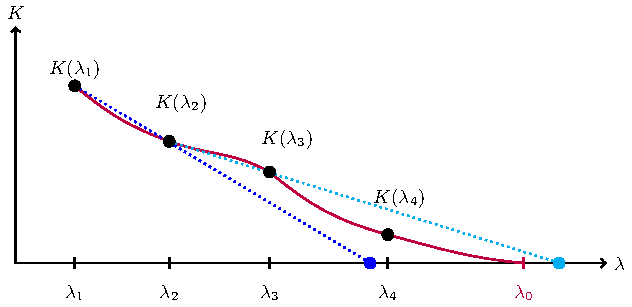
\includegraphics{NumFig1.pdf}\label{March}
\end{figure}

For example in Figure \ref{March}, the obvious choice for $\lambda_4$
(the light blue circle) is larger than the true value of $\lambda_0$, 
and therefore the naive extrapolation method won't quite work.
\clearpage
\section*{Guide to programs}
\subsection*{\color{blue} \texttt{K\_of\_c\_march}}
First the program sets up the spacing as $\tan^2$. It also sets the
initial $\bs{h}'= (\underbrace{1,\dots,1}_{g'} \underbrace{x_1+1, \dots,
x_n+1}_{h'})$ \textcolor{orange}{(Not sure why this is a reasonable first
guess, perhaps from the boundary conditions at $\infty$. Seems to have
no problems converging though.)}

Most of the work is then done by \texttt{fixed\_lambda\_M\_iteration}
which then solves for $K_I$ and $\bs{h}'$. 

N.B. $\bs{h}'$ is updated via $\displaystyle \bs{h}_i' = \frac{\bs{h}_{i-1}'
-\bs{h}_{i-2}'}{\lambda_{i-1} - \lambda_{i-2}} \lambda_i + 
\frac{\lambda_{i-1}\bs{h}_{i-2}'-\lambda_{i-1}\bs{h}_{i-1}'}
{\lambda_{i-1} - \lambda_{i-2}} $ which is just linear extrapolation.
In the absence of any better ideas this is the sensible choice.

After iterating for a few values, get near $\lambda_0$. Hear we suspect
that something like $K^3 \sim \lambda-\lambda_0$ near $\lambda=\lambda_0$,
$K=0$. So given two prior guesses, extrapolate via 
$\displaystyle \lambda_i = \frac{K_{i-1}^3\lambda_{i-2} - K_{i-2}^3
\lambda_{i-1}}{K_{i-1}^3-K_{i-2}^3}$ But as noted earlier, must be careful
to not extrapolate further than $\lambda_0$. So an idea is to take $(\lambda_i
+ \lambda_{i-1})/2$ as the next guess, i.e. 
\[\lambda_i = 
\frac{\lambda_{i-1} - \lambda_{i-2}}{K_{i-1}^3-K_{i-2}^3}\frac{K_{i-1}^3}{2}
+ \frac{K_{i-1}^3\lambda_{i-2} - K_{i-2}^3 
\lambda_{i-1}}{K_{i-1}^3-K_{i-2}^3} \]
Then the program just iterates. If it doesn't converge, it simply tries a 
smaller value of $\lambda$.

\subsection*{\color{blue} \texttt{fixed\_lambda\_M\_iteration}}
Takes a value of $\lambda$ and returns the corresponding $K$ value.
Now using the ``scaled'' version, so the values of $P,M$ are implicitly
assumed to be $0,1$ respectively.

\textcolor{red}{Somewhat concerningly, $\bs{h}'$ is assumed to 
already have this spacing, which could potentially cause issues.
If you wanted to change the spacing you would have to do it in
two different places.}

Subroutines then return the kernel matrix \& the interpolate matrix.
The kernel matrix is in lieu of $\displaystyle \left( \begin{array}{c}
p \\ 0 \end{array} \right) = \int \underline{\underline{K}} \left(
\begin{array}{c} g' \\ h' \end{array} \right) $.
The interpolate matrix actually only appears here to add in boundary
conditions to the matrix $A$.

The matrix $A$ is set up, which is part kernel, part interpolate matrix,
same matrix as described earlier.

The rcond statement is testing how conditioned the matrix $A$ is, or how 
ameniable it is to being numerically inverted. There does not seem to be
a huge amount of point in adding this step in.

Then the iteration loop begins. Follows Newton's method for the equation
$f(\bs{h}') = A \bs{h}'$ and iterates via $\displaystyle \bs{h}'_{new} =
\bs{h}'_{old} + (A-Df|_{\bs{h}_{old}'})^{-1}(f(\bs{h}_{old}') - A\bs{h}_{old}')$
Where we already know $A$. $f, Df$ are provided via \texttt{hprime\_to\_p}
and $f, Df$ are called $p, dp$ respectively in the program.

\end{document}
